\subsection{Structural Similarity Index (SSIM)}
Anders als die meisten anderen Vorgehensmodelle versucht die menschliche
Wahrnehmung nicht Fehler zu Quantifizieren, sondern strukturelle Informationen
aus einer Szene wiederzuerkennen. Um dieses Verhalten nachzuahmen, haben
Forschende Mitglieder der IEEE den Structual Similarity Index entworfen.
\parencite{ssim-orig-paper}

\noindent{Der Index extrahiert, vergleicht und kombiniert folgende drei
Parameter:}
\begin{itemize}[topsep=0pt]
    \item Leuchtdichte
    \item Kontrast
    \item Struktur
\end{itemize}

Im ersten Schritt wird die Leuchtdichte durch Mittelwertbildung über alle
Pixelwerte gemessen. Anschließend wird der Kontrast durch Berechnung der
Standardabweichung aller Werte ermittelt. Vereinfacht dargestellt wird die
Struktur durch die Teilung des Eingangssignals durch seine Standardabweichung
geteilt, sodass eine genormte Standardabweichung entsteht.
\parencite{ssim-summary}

Sobald die drei Werte berechnet wurden, werden diese anhand, im Original-Paper,
veröffentlichten mathematischen Funktionen verglichen und schließlich
kombiniert. \parencite{ssim-summary}

Obendrein sei es nützlich den Index nicht global auf das Bild anzuwenden. Das
Paper gibt an den Algorithmus vorzugsweise auf verschiedene lokale Stellen
einzusetzen. Erstens seien für die Analyse interessante Objekte oft instationär
und zweitens können Bildverzerrungen auch räumlich variabel sein. Um die
Referenz zur Nachahmung der menschlichen Wahrnehmung zu ziehen, ist ebenfalls
festzustellen, dass Menschen ebenfalls nur lokale Bereiche einer Grafik in hoher
Auflösung wahrnehmen können. \parencite{ssim-summary}

Auch wenn der SSIM durch seine Einfachheit, gegenüber anderen Verfahren, eine
überragende Performance aufweist, ist der Algorithmus sehr anfällig für
Skalierungen, Verschiebungen und Rotierungen (siehe Abbildung \ref{fig:ssim}).
\parencite{ssim-quality-assessment}

\begin{figure}[H]
    \centering
    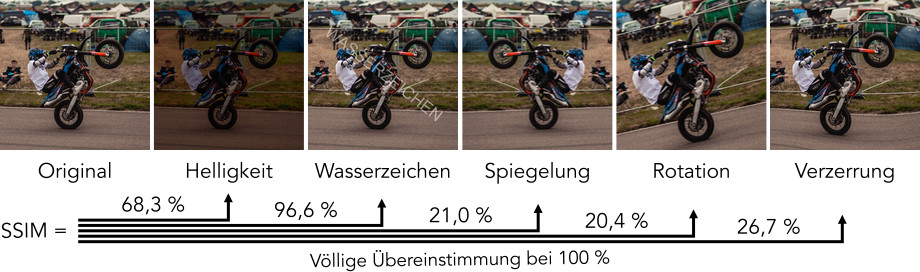
\includegraphics[width=\textwidth]{ssim}
    \caption{SSIM: Anwendung an verschiedenen Testbildern}
    \label{fig:ssim}
    \bildquelle{Eigene Darstellung}
\end{figure}


Aufbauend auf den SSIM-Algorithmus gibt es weitere optimierende Forschungen, wie
zum Beispiel der Complex Wavelet Structural Similarity Index. Der CW-SSIM
adressiert die vorher genannten Probleme und erzeugt durch Verwendung von
Wavelet-Transformationen eine Robustheit gegenüber kleinen Verschiebungen und
Rotierungen. \parencite{ssim-complex-wavelet}
